\documentclass[border=12pt]{standalone}
% shared preamble for all schematics/diagrams
\usepackage[siunitx, RPvoltages, european resistors]{circuitikz}
\usepackage{tikz}
\usetikzlibrary{arrows.meta,positioning,calc,shapes.geometric,fit,backgrounds,decorations.pathreplacing}
\usepackage[scaled=0.92]{helvet}
\renewcommand{\familydefault}{\sfdefault}
\usepackage{xcolor}
\usepackage{amsmath}
\usepackage{ifthen}
\definecolor{ink}{HTML}{1F2328}
\definecolor{muted}{HTML}{6B6A66}
\definecolor{c1}{HTML}{2A78D6}
\definecolor{c2}{HTML}{EB6834}
\definecolor{c3}{HTML}{1BAF7A}
\definecolor{c4}{HTML}{6250D6}
\definecolor{fill1}{HTML}{EAF2FC}
\definecolor{fill2}{HTML}{FDEEE7}
\definecolor{fill3}{HTML}{E6F6EF}
\definecolor{fill4}{HTML}{EFEDFB}
\definecolor{hv}{HTML}{C62828}
\ctikzset{bipoles/thickness=1.2, monopoles/ground/thickness=1.2}
\tikzset{every picture/.style={line width=0.7pt, color=ink}}

\begin{document}
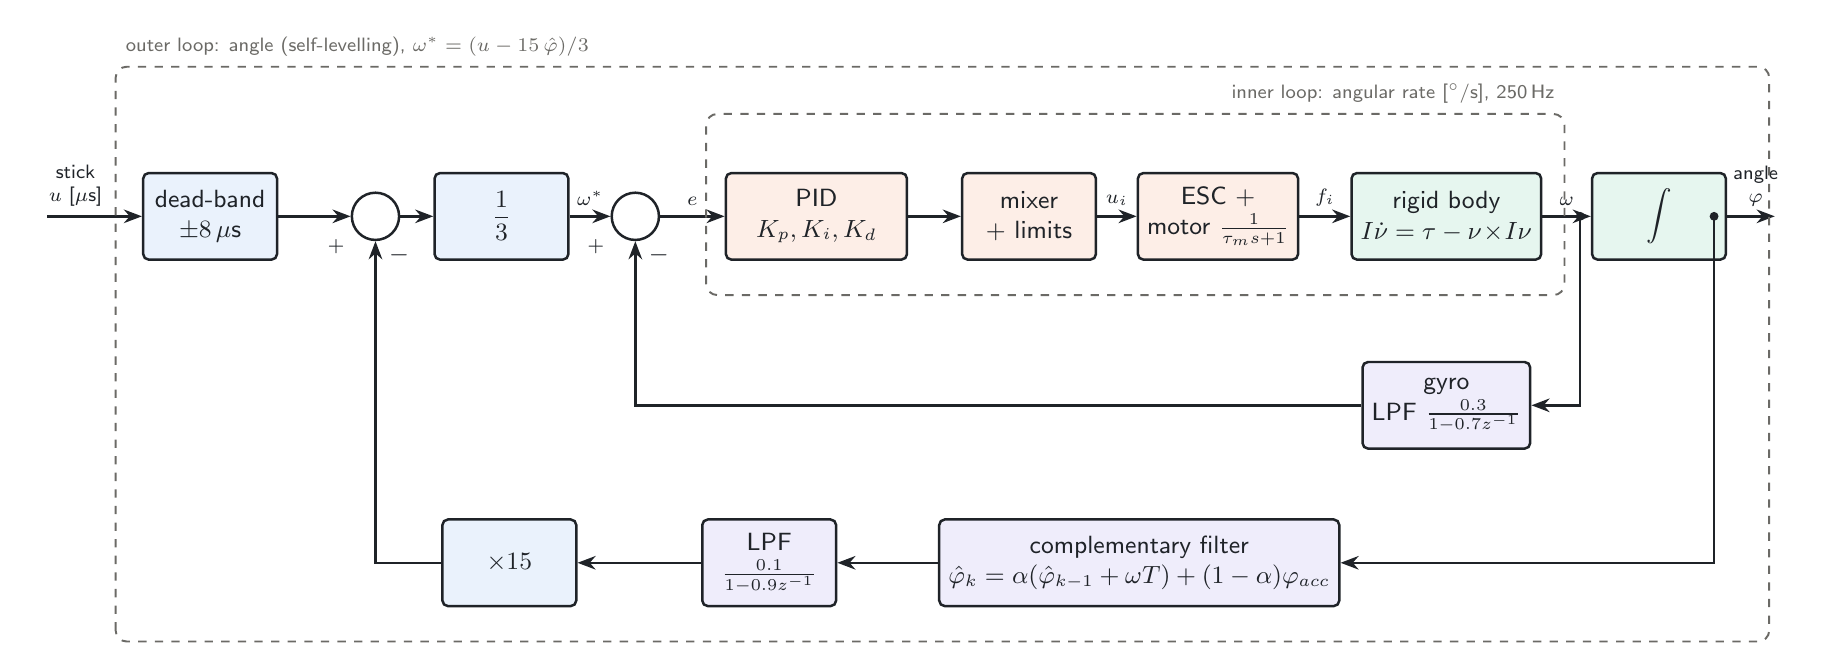
\begin{tikzpicture}[
  b/.style={draw, line width=0.9pt, fill=#1, minimum height=1.1cm, minimum width=1.7cm, align=center, font=\small, rounded corners=2pt},
  s/.style={draw, circle, line width=0.9pt, inner sep=0pt, minimum size=0.6cm, fill=white},
  a/.style={line width=0.9pt, -{Stealth[length=2.3mm]}},
  l/.style={font=\scriptsize, above, align=center}]
\node (in) at (0,0) {};
\node[b=fill1] (dz) at (2.2,0) {dead-band\\$\pm 8\,\mu$s};
\node[s] (s1) at (4.3,0) {};
\node[b=fill1] (k3) at (5.9,0) {$\dfrac{1}{3}$};
\node[s] (s2) at (7.6,0) {};
\node[b=fill2, minimum width=2.3cm] (pid) at (9.9,0) {PID\\$K_p, K_i, K_d$};
\node[b=fill2] (mix) at (12.6,0) {mixer\\+ limits};
\node[b=fill2] (esc) at (15.0,0) {ESC +\\motor $\frac{1}{\tau_m s+1}$};
\node[b=fill3, minimum width=2.4cm] (body) at (17.9,0) {rigid body\\$I\dot\nu = \tau - \nu\!\times\! I\nu$};
\node[b=fill3] (int) at (20.6,0) {$\displaystyle\int$};
\node (out) at (22.2,0) {};
\draw[a] (in) -- (dz) node[l, pos=0.3] {stick\\$u$ [$\mu$s]};
\draw[a] (dz) -- (s1);
\draw[a] (s1) -- (k3);
\draw[a] (k3) -- (s2) node[l, midway] {$\omega^*$};
\draw[a] (s2) -- (pid) node[l, midway] {$e$};
\draw[a] (pid) -- (mix);
\draw[a] (mix) -- (esc) node[l, midway] {$u_i$};
\draw[a] (esc) -- (body) node[l, midway] {$f_i$};
\draw[a] (body) -- (int) node[l, midway] {$\omega$};
\draw[a] (int) -- (out) node[l, pos=0.6] {angle\\$\varphi$};
% rate feedback
\node[b=fill4] (gyro) at (17.9,-2.4) {gyro\\LPF $\frac{0.3}{1-0.7z^{-1}}$};
\draw[a] (19.6,0) |- (gyro.east); \fill (19.6,0) circle (1.6pt);
\draw[a] (gyro.west) -| (s2);
\node[font=\scriptsize] at (7.1,-0.38) {$+$}; \node[font=\small] at (7.9,-0.5) {$-$};
% angle feedback
\node[b=fill4, minimum width=3.2cm] (cf) at (14.0,-4.4) {complementary filter\\$\hat\varphi_k = \alpha(\hat\varphi_{k-1}+\omega T) + (1-\alpha)\varphi_{acc}$};
\node[b=fill4] (lp) at (9.3,-4.4) {LPF\\$\frac{0.1}{1-0.9z^{-1}}$};
\node[b=fill1] (k15) at (6.0,-4.4) {$\times 15$};
\draw[a] (21.3,0) |- (cf.east); \fill (21.3,0) circle (1.6pt);
\draw[a] (cf) -- (lp);
\draw[a] (lp) -- (k15);
\draw[a] (k15.west) -| (s1);
\node[font=\scriptsize] at (3.8,-0.38) {$+$}; \node[font=\small] at (4.6,-0.5) {$-$};
\draw[dashed, muted, rounded corners] (8.5,-1.0) rectangle (19.4,1.3);
\node[font=\scriptsize, muted, anchor=south east] at (19.4,1.3) {inner loop: angular rate [$^\circ$/s], 250\,Hz};
\draw[dashed, muted, rounded corners] (1.0,-5.4) rectangle (22.0,1.9);
\node[font=\scriptsize, muted, anchor=south west] at (1.0,1.9) {outer loop: angle (self-levelling), $\omega^* = (u - 15\,\hat\varphi)/3$};
\end{tikzpicture}
\end{document}
